\documentclass[]{politex}
% ========== Opções ==========
% pnumromarab - Numeração de páginas usando algarismos romanos na parte pré-textual e arábicos na parte textual
% abnttoc - Forçar paginação no sumário conforme ABNT (inclui "p." na frente das páginas)
% normalnum - Numeração contínua de figuras e tabelas
%	(caso contrário, a numeração é reiniciada a cada capítulo)
% draftprint - Ajusta as margens para impressão de rascunhos
%	(reduz a margem interna)
% twosideprint - Ajusta as margens para impressão frente e verso
% capsec - Forçar letras maiúsculas no título das seções
% espacosimples - Documento usando espaçamento simples
% espacoduplo - Documento usando espaçamento duplo
%	(o padrão é usar espaçamento 1.5)
% times - Tenta usar a fonte Times New Roman para o corpo do texto
% noindentfirst - Não indenta o primeiro parágrafo dos capítulos/seções


% ========== Packages ==========
\usepackage[utf8]{inputenc}
\usepackage{amsmath,amsthm,amsfonts,amssymb}
\usepackage{float}
\usepackage{graphicx,hyperref,cite,enumerate}


% ========== Language options ==========
\usepackage[brazil]{babel}
%\usepackage[english]{babel}


% ========== ABNT (requer ABNTeX 2) ==========
%	http://www.ctan.org/tex-archive/macros/latex/contrib/abntex2
\usepackage[alf]{abntex2cite}

% Forçar o abntex2 a usar [ ] nas referências ao invés de ( )
%\citebrackets{[}{]}


% ========== Lorem ipsum ==========
\usepackage{blindtext}

% ========== PATH Relativo das Imagens ==========
\graphicspath{ {imagens/} }

% ========== Opções do documento ==========
% Título
\titulo{Sistema de Gerenciamento de Disciplinas de Projeto de Formatura do PCS}

% Autor
\autor{Lucas Arthur Felgueiras}

% Para múltiplos autores (TCC)
%\autor{Nome Sobrenome\\%
%		Nome Sobrenome\\%
%		Nome Sobrenome}

% Orientador / Coorientador
\orientador{Prof. Dr. Fabio Levy Siqueira}
% \coorientador{Nome do coorientador (opcional)}

% Tipo de documento
\tcc{de Computação}
%\dissertacao{Engenharia Elétrica}
%\teseDOC{Engenharia Elétrica}
%\teseLD
%\memorialLD

% Departamento e área de concentração
\departamento{Engenharia de Computação e Sistemas Digitais}
\areaConcentracao{Engenharia de Software}

% Local
\local{São Paulo}

% Ano
\data{2018}




\begin{document}
% ========== Capa e folhas de rosto ==========
\capa
\falsafolhaderosto
\folhaderosto


% ========== Folha de assinaturas (opcional) ==========
%\begin{folhadeaprovacao}
%	\assinatura{Prof.\ X}
%	\assinatura{Prof.\ Y}
%	\assinatura{Prof.\ Z}
%\end{folhadeaprovacao}


% ========== Ficha catalográfica ==========
% Fazer solicitação no site:
%	http://www.poli.usp.br/en/bibliotecas/servicos/catalogacao-na-publicacao.html


% ========== Dedicatória (opcional) ==========
\dedicatoria{Dedicatória}


% ========== Agradecimentos ==========
\begin{agradecimentos}

Thanks...

\end{agradecimentos}


% ========== Epígrafe (opcional) ==========
\epigrafe{%
	\emph{``Epígrafe''}
	\begin{flushright}
		-{}- Autor
	\end{flushright}
}


% ========== Resumo ==========
\begin{resumo}
Resumo...
%
\\[3\baselineskip]
%
\textbf{Palavras-Chave} -- Palavra, Palavra, Palavra, Palavra, Palavra.
\end{resumo}


% ========== Abstract ==========
\begin{abstract}
Abstract...
%
\\[3\baselineskip]
%
\textbf{Keywords} -- Word, Word, Word, Word, Word.
\end{abstract}


% ========== Listas (opcional) ==========
\listadefiguras
\listadetabelas

% ========== Listas definidas pelo usuário (opcional) ==========
% \begin{pretextualsection}{Lista de símbolos}

% Lista de símbolos...

% \end{pretextualsection}

% ========== Sumário ==========
\sumario



% ========== Elementos textuais ==========

\chapter{Introdução}
\section{Motivação}
\section{Objetivo}
\section{Justificativa}
\section{Organização do Trabalho}

\chapter{Aspectos Conceituais}
\section{Levantamento de Requisitos}
Em Engenharia de Software, é essencial o momento do levantamento de requisitos, dado que são eles que ditam o funcionamento do software a ser desenvolvido, alinha as expectativas dos \textit{stakeholders} e determinam os requisitos funcionais e não funcionais necessários para a aceitação. Neste projeto, para o levantamento de requisitos, foi usada uma das técnicas descritas em \cite{kurtbittnerianspence2002}, que consiste em levantar primeiramente os \textit{stakeholders} do projeto. Segundo \cite{kurtbittnerianspence2002}, a definição traduzida de \textit{stakeholder} é a seguinte:

\begin{citacaoLonga}
"Um indivíduo que é materialmente afetado pelo resultado do
sistema ou o(s) projeto(s) que produzem o sistema."
\end{citacaoLonga}

Ou seja, \textit{stakeholders} não são apenas os indivíduos que efetivamente usarão o sistema, mas sim todos os impactados sua existência. O livro divide os \textit{stakeholders} em 5 grupos:

\begin{itemize}
    \item Usuários: as pessoas que efetivamente usarão o sistema.
    \item Patrocinadores: os financiadores do projeto de software que gerará o sistema.
    \item Desenvolvedores: os responsáveis por desenvolver o sistema levantado pelo processo.
    \item Autoridades: órgãos reguladores que determinam regras para o uso de determinado software.
    \item Consumidores: empresas que compram esses softwares para serem usados.
\end{itemize}

\subsection{Entendimento dos Problemas}

Uma vez mapeado os \textit{stakeholders}, partimos para entender agora as dores que cada um possui e o que eles esperam com o produto final a ser desenvolvido. Alguns processos são sugeridos pelo livro\cite{kurtbittnerianspence2002}, como por exemplo:

\begin{itemize}
    \item Entrevistas: entrevistar os envolvidos e entender diretamente quais são suas dores e expectativas.
    \item Questionários: São úteis quando há um amplo número de \textit{stakeholders} envolvidos.
    \item Grupo Focal: Reunião com alguns representantes dos grupos de \textit{stakeholders} para entender e construir uma visão única sobre o projeto.
    \item Quadros de Aviso: É um tipo particular de grupo focal, onde o quadro serve como unificador da visão, com a diferença de não ter todos reunidos ao mesmo tempo.
    \item \textit{Workshops}: Eventos avisados com antecedência para entender melhor sobre o sistema, com a participação dos envolvidos.
    \item Revisões: Reuniões informais com o intuito de revisar documentos gerados com alguns envolvidos.
    \item Encenação: É uma técnica facilitadora usada em conjunto com \textit{workshops} para obter informações mais específicas ou \textit{feedbacks}.
\end{itemize}

Com essa listagem de problemas levantados pelos processos de levantamento de requisitos, finalmente podemos partir para a visão unificada do processo como um todo e como o software vai atuar no processo. Para isso, é saudável a elaboração de um documento unificando os pontos de vista dos \textit{stakeholders} e estabelecendo o que de fato será o sistema a ser desenvolvido, resultando no Documento de Visão.

\subsection{Documento de Visão}

O documento de visão, segundo o livro\cite{kurtbittnerianspence2002}, traz a seguinte definição (traduzida):

\begin{citacaoLonga}
O Documento de Visão é o artefato do Rational Unified Process\cite{ibm2011} que capta todas as informações de requisitos. Como toda documentação de requisitos, seu objetivo principal é a comunicação.
\end{citacaoLonga}

Existem diversos modelos de Documento de Visão, porém, em sua essência, atendem os seguintes tópicos\cite{kurtbittnerianspence2002}:

\begin{enumerate}
    \item Posicionamento: Como o sistema irá se posicionar no quesito de negócios? Há concorrentes que já resolvem o problema? Quais são seus diferenciais em relação a eles?
    \item \textit{Stakeholders} e usuários: Quem são os envolvidos direta e indiretamente com o desenvolvimento e a existência do sistema?
    \item Necessidades chave: Quais são as demandas que realmente precisam estar nos planos do sistema para satisfazer os envolvidos?
    \item Visão geral do produto: O que é o produto de fato? Quais são suas dependências, capacidades e alternativas ao seu desenvolvimento?
    \item Funcionalidades: Quais são as funcionalidades em alto nível do sistema, para que elas resolvam as necessidades chave listadas anteriormente?
    \item Outros requisitos do produto: Quais são os outros requisitos do sistema que não foram capturados como funcionalidades?
\end{enumerate}

\section{Histórias de Usuário}

Uma das abordagens possíveis para se estabelecer os requisitos levantados e começar a desenvolver de fato o sistema é o uso de Histórias de Usuários (ou \textit{User Stories}). A definição de Histórias de Usuário, traduzido de \cite{jonathanrasmusson}, está a seguir:

\begin{citacaoLonga}
São descrições curtas das funcionalidades que o nosso cliente
gostaria de um dia ver em seu software. Eles geralmente são escritos em pequenos cartões de índice (para nos lembrar de não tentar escrever tudo) e estão lá para nos encorajar a ir falar com nossos clientes.
\end{citacaoLonga}

\subsection{Escopo base da história}
O essencial em escrever boas histórias de usuário está em agregar valor para os \textit{stakeholders}. Ou seja, escrever histórias de usuário que tangem assuntos como arquitetura do sistema, linguagem de implementação, padrões de código entre outros não são boas histórias de usuário, pois salvo raríssimas exceções, o cliente não vê valor em histórias desse tipo.

Em contrapartida, histórias sobre o comportamento do sistema que carregam valor de produto nelas são histórias de usuário importantes para o processo de desenvolvimento. Muitas vezes, porém, histórias de usuário forçam um viés altamente técnico; nessas situações, cabe buscar a causa raiz que levou à "solução" escrita na história: histórias de usuário apresentam problemas de negócio, jamais soluções técnicas.

\subsection{Características básicas}

Boas histórias de usuário costumam ser independentes entre si. Tal independência é importantíssima para mudanças no projeto (que ocorrem com frequência), porque histórias isoladas são fáceis de serem alteradas. Outro ponto importante está em elas serem negociáveis, ou seja, elas podem sofrer alterações e inclusive serem removidas se, com o andamento do projeto, ela perder sua prioridade e tais alterações e remoções não afetam o andar geral das outras tarefas.

Por fim, elas precisam de mais duas características fundamentais: precisam ser testáveis (e quantificar esses testes, se possível), tanto no fluxo de negócio como na escrita de testes automatizados, assim podemos garantir com facilidade a qualidade do que está sendo entregue e; precisam ser pequenas e estimáveis, ou seja, o esforço dela pode ser previsto com antecedência (essa por projetos anteriores ou pela experiência dos integrantes da equipe), permitindo assim medidas de performance dos envolvidos, escopo entregue, entre outros.

\subsection{Um padrão para Histórias de Usuário}

Um bom padrão para escrever histórias de usuário está a seguir\cite{jonathanrasmusson}:

\begin{citacaoLonga}
Eu como $<$para quem é a história$>$
\\
Eu quero $<$o que ele quer$>$
\\
por causa $<$por que ele quer$>$
\end{citacaoLonga}

\section{Casos de Uso}

Como outra alternativa para documentar o que será desenvolvido no sistema, há a solução clássica de desenvolvimento de software: casos de uso. Essencialmente, cada caso de uso possui um ou mais atores agindo com o sistema. Segundo as definições traduzidas de \cite{kurtbittnerianspence2002}:

\begin{citacaoLonga}
\textbf{Atores} representam as pessoas ou coisas que interagem de alguma forma com o sistema; por definição, eles estão fora do sistema. Eles têm um nome e uma breve descrição, e eles estão associados com os casos de uso com os quais eles interagem.
\\
\\
\textbf{Casos de Uso} representam as coisas de valor que o sistema executa para os atores. Casos de uso não são funções ou recursos e não podem ser decompostos. Casos de uso têm um nome e uma breve descrição. Eles também tem descrições detalhadas que são essencialmente histórias sobre como o atores usam o sistema para fazer algo que considerem importante, e que o sistema faz para satisfazer essas necessidades.
\end{citacaoLonga}

\subsection{Características básicas}
Casos de uso, como escrito acima, descrevem as interações entre os atores e o sistema projetado, logo, é coerente que eles estejam relacionados à um processo completo, com começo, meio e fim. Uma grande vantagem de uso dessa técnica está em estabelecer uma espécie de contrato entre a equipe de concepção do sistema e os \textit{stakeholders}, o que evita a participação constante dos envolvidos durante o desenvolvimento.

Um fator interessante está na concepção do documento dos casos de uso, pois ela pode ocorrer de duas formas: como um documento resultante do documento de visão, gerado durante o levantamento de requisitos, ou como uma estratégia para levantar os requisitos e, como consequência, gerar o documento de visão\cite{elisayuminakagawa2013}.

\subsection{Uma estrutura de caso de uso}
Essencialmente, um caso de uso deve possuir a seguinte estrutura\cite{funpar2001}, baseada em \cite{ibm2011}:

\begin{enumerate}
    \item Nome: Nome do Caso de Uso
    \begin{enumerate}
        \item Breve Descrição: Finalidade do caso de uso
    \end{enumerate}
    \item Fluxo de Eventos: A descrição dos eventos que ocorrem no sistema, que são divididos em dois conjuntos principais.
    \begin{enumerate}
        \item Fluxo Básico: É o comportamento básico da interação entre os atores e o sistema. Aqui não devemos ter situações de contorno nem exceções, isso fica ao encargo dos fluxos alternativos.
        \item Fluxos Alternativos: Comportamentos diferenciados do caso de uso, podendo haver mais de um.
    \end{enumerate}
    \item Requisitos Especiais: Requisito não funcional que é específico de um caso de uso, mas que não está contemplado no fluxo de eventos.
    \item Pré-condição: Estado do sistema antes da realização do caso de uso.
    \item Pós-condição: Possíveis estados do sistema após a execução do caso de uso.
\end{enumerate}

Essa estrutura é interessante, pois atende o que deve ser um caso de uso: deve fugir de uma estrutura pequena, englobando um fluxo bem definido do sistema e que traga valor de negócio para os envolvidos. Além disso, com sua descrição comportamental, ele serve como um contrato estabelecido de desenvolvimento, o que abona a participação integral dos \textit{stakeholders}, como é de se esperar de um caso de uso.

\section{Verificação e Validação}

Durante o desenvolvimento, é saudável garantir a qualidade do que está sendo entregue, tanto na parte técnica, quanto no alinhamento com a parte de negócios do projeto. Para isso, existem os processos de verificação e validação, traduzidos do SWEBOK\cite{ieeecomputersociety2014}:

\begin{citacaoLonga}
O objetivo da verificação e validação é ajudar a equipe de desenvolvimento a garantir qualidade no sistema por todo seu ciclo de vida.
\end{citacaoLonga}

\subsection{Verificação}
Em desenvolvimento de software, é uma boa prática acompanhar se os requisitos funcionais e não funcionais estão sendo atendidos, de preferência com acompanhamento das métricas determinadas nos requisitos. Essa prática é conhecida como verificação, definida de maneira resumida pela seguinte pergunta\cite{eduardofigueiredo2018}:

\begin{citacaoLonga}
Estamos construindo o produto corretamente?
\end{citacaoLonga}

\subsection{Validação}
Além de acompanhar os requisitos propostos, é importante entender se o sistema está de acordo com as expectativas operacionais dos \textit{stakeholders}. Essa análise constante de adequação voltada aos negócios é conhecida como validação, definida pela seguinte questão\cite{eduardofigueiredo2018}:

\begin{citacaoLonga}
Estamos construindo o produto correto?
\end{citacaoLonga}

\subsection{Testes}
Em ambos os casos descritos acima, é necessário ter uma ferramenta que automatize esses processos e permita manter a consistência do que foi entregue quando há novas funcionalidades a serem lançadas. Para isso, existe o conceito de testes, onde o sistema passa por uma bateria de exames e revisões para detectar erros e garantir a qualidade e alinhamento do que foi entregue. Vale lembrar que essa bateria de testes é finita, sendo um subgrupo dos infinitos fluxos de execução do domínio\cite{ieeecomputersociety2014}.

Na escala macroscópica, temos os testes de aceitação junto aos \textit{stakeholders}, para validar a conformidade dos requisitos e a qualidade das entregas. Já para testar a arquitetura, costumam ser realizados testes de sistema. Para testar os componentes desenvolvidos do sistema, realizam-se testes de integração entre esses componentes. E, por fim, o código escrito para cada componente elaborado é testado pelos testes de unidade.

\begin{figure}[H]
    \centering
    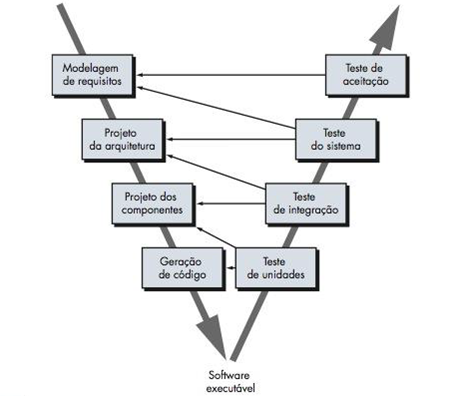
\includegraphics[scale=0.90]{modelo-v.png}
    \caption{Estrutura de Testes Modelo V\cite{devmedia2013}}
    \label{fig:modelo-v}
\end{figure}

Ao desenvolver um sistema, cada teste deve ser executado a cada nova funcionalidade adicionada e/ou modificada, pois só assim é possível garantir a qualidade do que já foi entregue. Uma boa prática para realizar esses testes, em especial os testes menores, é automatizar a execução deles, o que economiza tempo de uma pessoa dedicada à função de testador.


\chapter{Tecnologias Utilizadas}
\section{\textit{Frameworks web}}

É comum, em desenvolvimento de sistemas, usar soluções prontas como forma de simplificar o desenvolvimento de soluções mais avançadas. Em especial, na área de aplicações \textit{web}, é uma solução desejável pois além de acelerar o desenvolvimento, usa-se uma solução amplamente testada no mercado e de confiança para aplicações comerciais. Tais soluções prontas são chamadas de arcabouços (ou \textit{frameworks}). Para este projeto, não foi diferente: por motivos de agilidade, mesclados com requisitos de manutenibilidade do sistema, foi escolhido um \textit{framework} em linguagem Python, chamado \textbf{Django}.

\subsection{Django}
O Django teve sua primeira versão lançada em Setembro de 2008\cite{djangowikispaces2012}, contendo muito do que é encontrado atualmente na versão 2.1\cite{djangodocs}: padrão \textit{Model-View-Controller}, gerenciamento de banco de dados eficiente, padrões para roteamento de URLs, entre outras funcionalidades. O \textit{framework} nasceu de uma empresa de desenvolvimento de sistemas para jornalismo, onde os prazos são frequentes e, muitas vezes, inegociáveis, logo, surgiu uma necessidade de uma solução rápida de implementar e estável para aplicações comerciais, resultando no nascimento do Django\cite{djangogeneral2018}.

O Django é estruturado em aplicações (apps), onde cada aplicação corresponde a uma parte do sistema, geralmente independente e reciclável (ou seja, pode ser usada em aplicações Django diferentes). Cada aplicação segue o padrão \textit{Model-View-Controller}, que será explicado melhor adiante\cite{djangodocs}. Hoje, sua versão mais recente estável é a 2.1, que corrigiu algumas novidades da versão 2.0. É esta versão que foi usada pelo projeto em questão, dado que é estável e possui suporte de apoio da equipe até Dezembro de 2020\cite{djangodownload}.

\subsection{Padrão \textit{Model-View-Controller}}
O padrão \textit{Model-View-Controller} - MVC (ou \textit{Model-Template-View} - MTV) consiste em um padrão arquitetural de software para organizar os componentes da aplicação de maneira eficiente e de fácil manutenção. Há diversos outros padrões arquiteturais (como por exemplo a arquitetura em camadas), mas o caso do Django é explícito o uso desse padrão.

Este padrão é dividido em três grandes grupos\cite{thedjangobook2018}:

\begin{itemize}
    \item Modelo (\textit{Model}): Uma representação (interface) para os dados da aplicação.
    \item Visualização (\textit{View}): Camada de apresentação dos dados da aplicação. No caso do Django, está mais alinhado com o \textit{Template}.
    \item Controlador (\textit{Controller}): Camada de controle que interliga o modelo com a apresentação dos dados, onde geralmente fica a lógica de negócio. No caso do Django, está mais alinhado com a \textit{View}.
\end{itemize}

\begin{figure}[H]
    \centering
    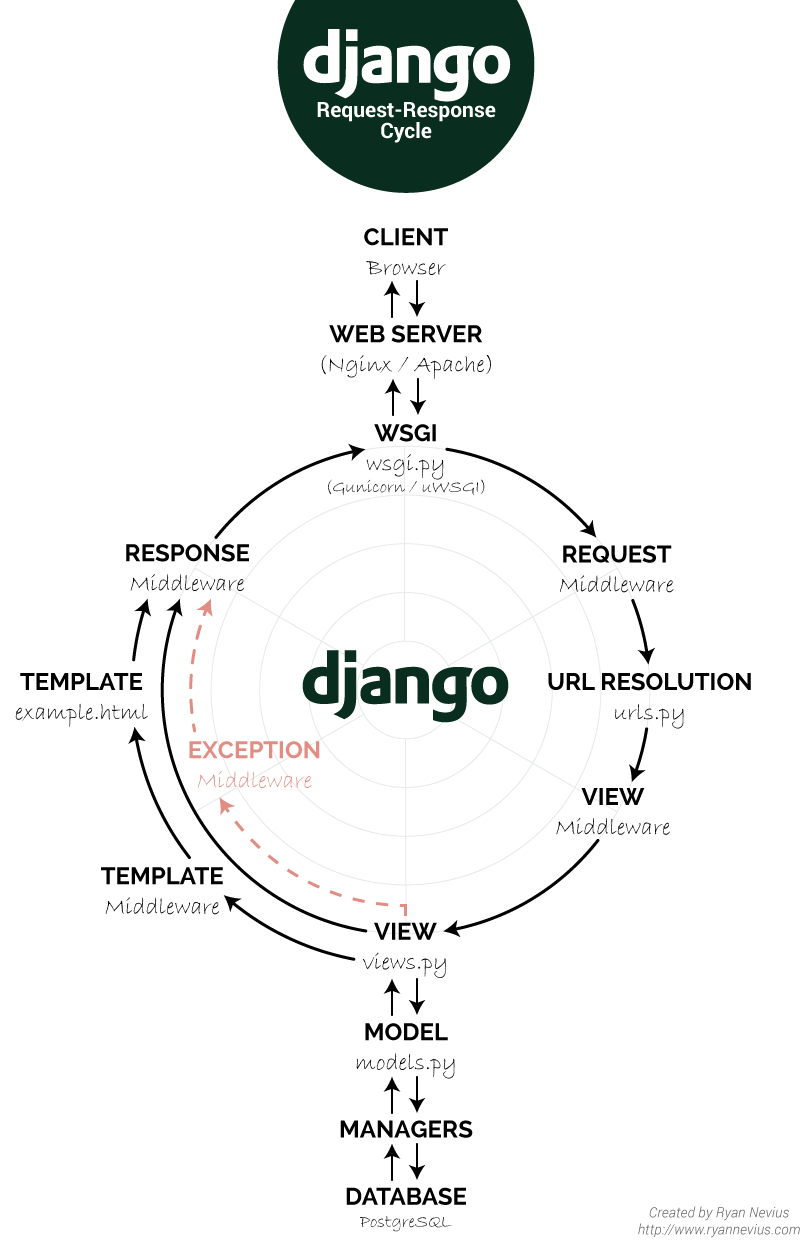
\includegraphics[scale=0.20]{model-view-template.png}
    \caption{Arquitetura MTV do Django\cite{codelv2018}}
    \label{fig:mtv-django}
\end{figure}

A vantagem do padrão está no fluxo de dados evidente que existe entre as camadas, além de evitar códigos com funcionalidades diferentes em lugares errados, como por exemplo lógica de negócio na camada de apresentação.

\section{Banco de Dados}

Assim como em projetos grandes de sistemas, o uso de banco de dados tornou-se necessário no projeto em questão. Porém, hoje possuímos diversos tipos e estruturas de bancos de dados distintos e, de acordo com os requisitos de um projeto, é tomada a decisão de qual é o melhor banco a ser usado no contexto. Segundo a definição traduzida do dicionário de Cambridge\cite{cambridgeuniversitypress2018}, o significado comercial de Banco de Dados é:

\begin{citacaoLonga}
Um sistema de computador que contém uma grande quantidade de informações que podem ser visualizadas ou alteradas facilmente.
\end{citacaoLonga}

Essencialmente, um banco de dados é uma coleção de informações organizadas, estruturadas ou não, guardadas em um computador e usadas para os mais diversos fins. Para acessar essas informações, usam-se sistemas para controlar a consulta a essas informações, tanto do lado do usuário final, como do lado dos desenvolvedores. Esses sistemas são conhecidos como Sistemas de Gerenciamento de Banco de Dados (SGBD)\cite{devmedia2014}.

Há diversos tipos de banco de dados no mercado, porém, para o projeto, foi adotado o modelo clássico relacional.

\subsection{Bancos Relacionais}
Bancos de dados relacionais são bancos onde cada coletânea de dados pode possuir uma relação pré-estabelecida. Para isso, é comum a estruturação deles por meio de tabelas, onde cada coluna é um tipo de dado e a linha é o valor em si. Cada linha é marcada com o que é chamado de chave primária, e é por meio dela que é possível fazer referência desse dado em outras tabelas. Para auxiliar as consultas e operações nesses bancos, bancos relacionais costumam usar uma linguagem própria para realizar tais operações, conhecida como Linguagem de Consulta Estruturada (Structured Query Language - SQL). O SQL foi determinado como padrão em 1986 e, desde então, é usado com pequenas variações entre os mais diversos mecanismos de banco de dados relacionais\cite{amazonwebservices2018}.

\subsubsection{SQLite}
O SQLite é um SGBD implementado em C, com o diferencial de ser leve e embutido na própria aplicação, ou seja, o banco fica junto com a aplicação carregada. A principal vantagem está em sua simplicidade, dado que o banco praticamente está pronto para ser usado pelo sistema. A desvantagem está no acoplamento entre o banco e a aplicação, o que nem sempre é saudável\cite{devmedia2007}.

\subsubsection{PostgreSQL}
O PostgreSQL é outro tipo de SGBD, bem mais robusto que o exemplo anterior, dado que é um servidor real dedicado para realizar a gestão de dados. Ele é mais preparado para lidar com cargas de trabalho maiores, consultas mais pesadas, entre outras tarefas robustas. Além disso, possui uma segurança mais reforçada, técnicas de recuperação de dados, entre outros. Como principal desvantagem, temos a complexidade para configurar e manter esse banco como infraestrutura dependente do projeto, o que, em casos de projetos simples, pode ser trabalho desnecessário\cite{devmedia2015}.

\subsection{Decisões de Projeto}
No âmbito de banco de dados relacional, o Django usa como padrão o SQLite, o que atendeu bem durante o desenvolvimento. Já o Heroku tem como banco de dados padrão o PostgreSQL, o que exigiu o chaveamento entre os bancos no ambiente local de desenvolvimento e os ambientes de validação hospedados no serviço. Por isso, o projeto possui configurado dois pacotes de gerenciamento de banco de dados, um para SQLite (nativo do Django), outro para PostgreSQL (o Psycopg\cite{lucassouto2017}).

\section{Ambientes de Validação}
É uma boa prática, para desenvolvimento de sistemas, criar diversos ambientes de aplicação, para validar as funcionalidades desenvolvidas tanto com a equipe de desenvolvimento, como com os \textit{stakeholders}, fora o ambiente onde a aplicação será hospedada, de fato (ou seja, onde ela ficará em ambiente de produção). Cada sistema exige 1 ou mais ambientes durante o fluxo de desenvolvimento, de acordo com a complexidade de negócios do projeto. Durante este capítulo, será explicitado mais sobre como foi estruturado os ambientes de teste e quais tecnologias de apoio foram usadas.

\subsection{Organização Genérica}
Para o projeto, foram organizados três ambientes de aplicação para realizar os processos de validação e homologação do sistema, para permitir testes isolados dos \textit{stakeholders} sem afetar o fluxo de desenvolvimento. São eles: Desenvolvimento (ou \textit{next-release}), Homologação (ou \textit{staging}) e Produção (ou \textit{production})\cite{ilyasabanin2018}.

\subsubsection{Desenvolvimento}
No ambiente de desenvolvimento, sempre fica a versão mais recente e estável da aplicação, com as novas funcionalidades desenvolvidas e testadas já integradas no ambiente. Essa versão serve como uma prévia do que será entregue para homologação. As mudanças nesse ambiente são mais frequentes, dado que uma nova funcionalidade completa já pode ir para este ambiente.

\subsubsection{Homologação}
Já neste ambiente, as mudanças são bem menores e servem como ambiente de aprovação dessas mudanças por parte dos \textit{stakeholders}. No caso do sistema de TCCs, ele serviu como homologação com os coordenadores do curso. Se possível, ele deve ser o mais fiél ao ambiente final de produção, assim o comportamento ideal dele em homologação será o mesmo em produção.

\subsubsection{Produção}
Já este ambiente é onde o sistema irá rodar, de fato. Esse ambiente deve ser o mais estável possível, com alterações apenas homologadas pelos \textit{stakeholders}. Salvo raras exceções, como falhas e problemas encontrados, nada deve ser colocado aqui sem a aprovação no ambiente de homologação.

\begin{figure}[H]
    \centering
    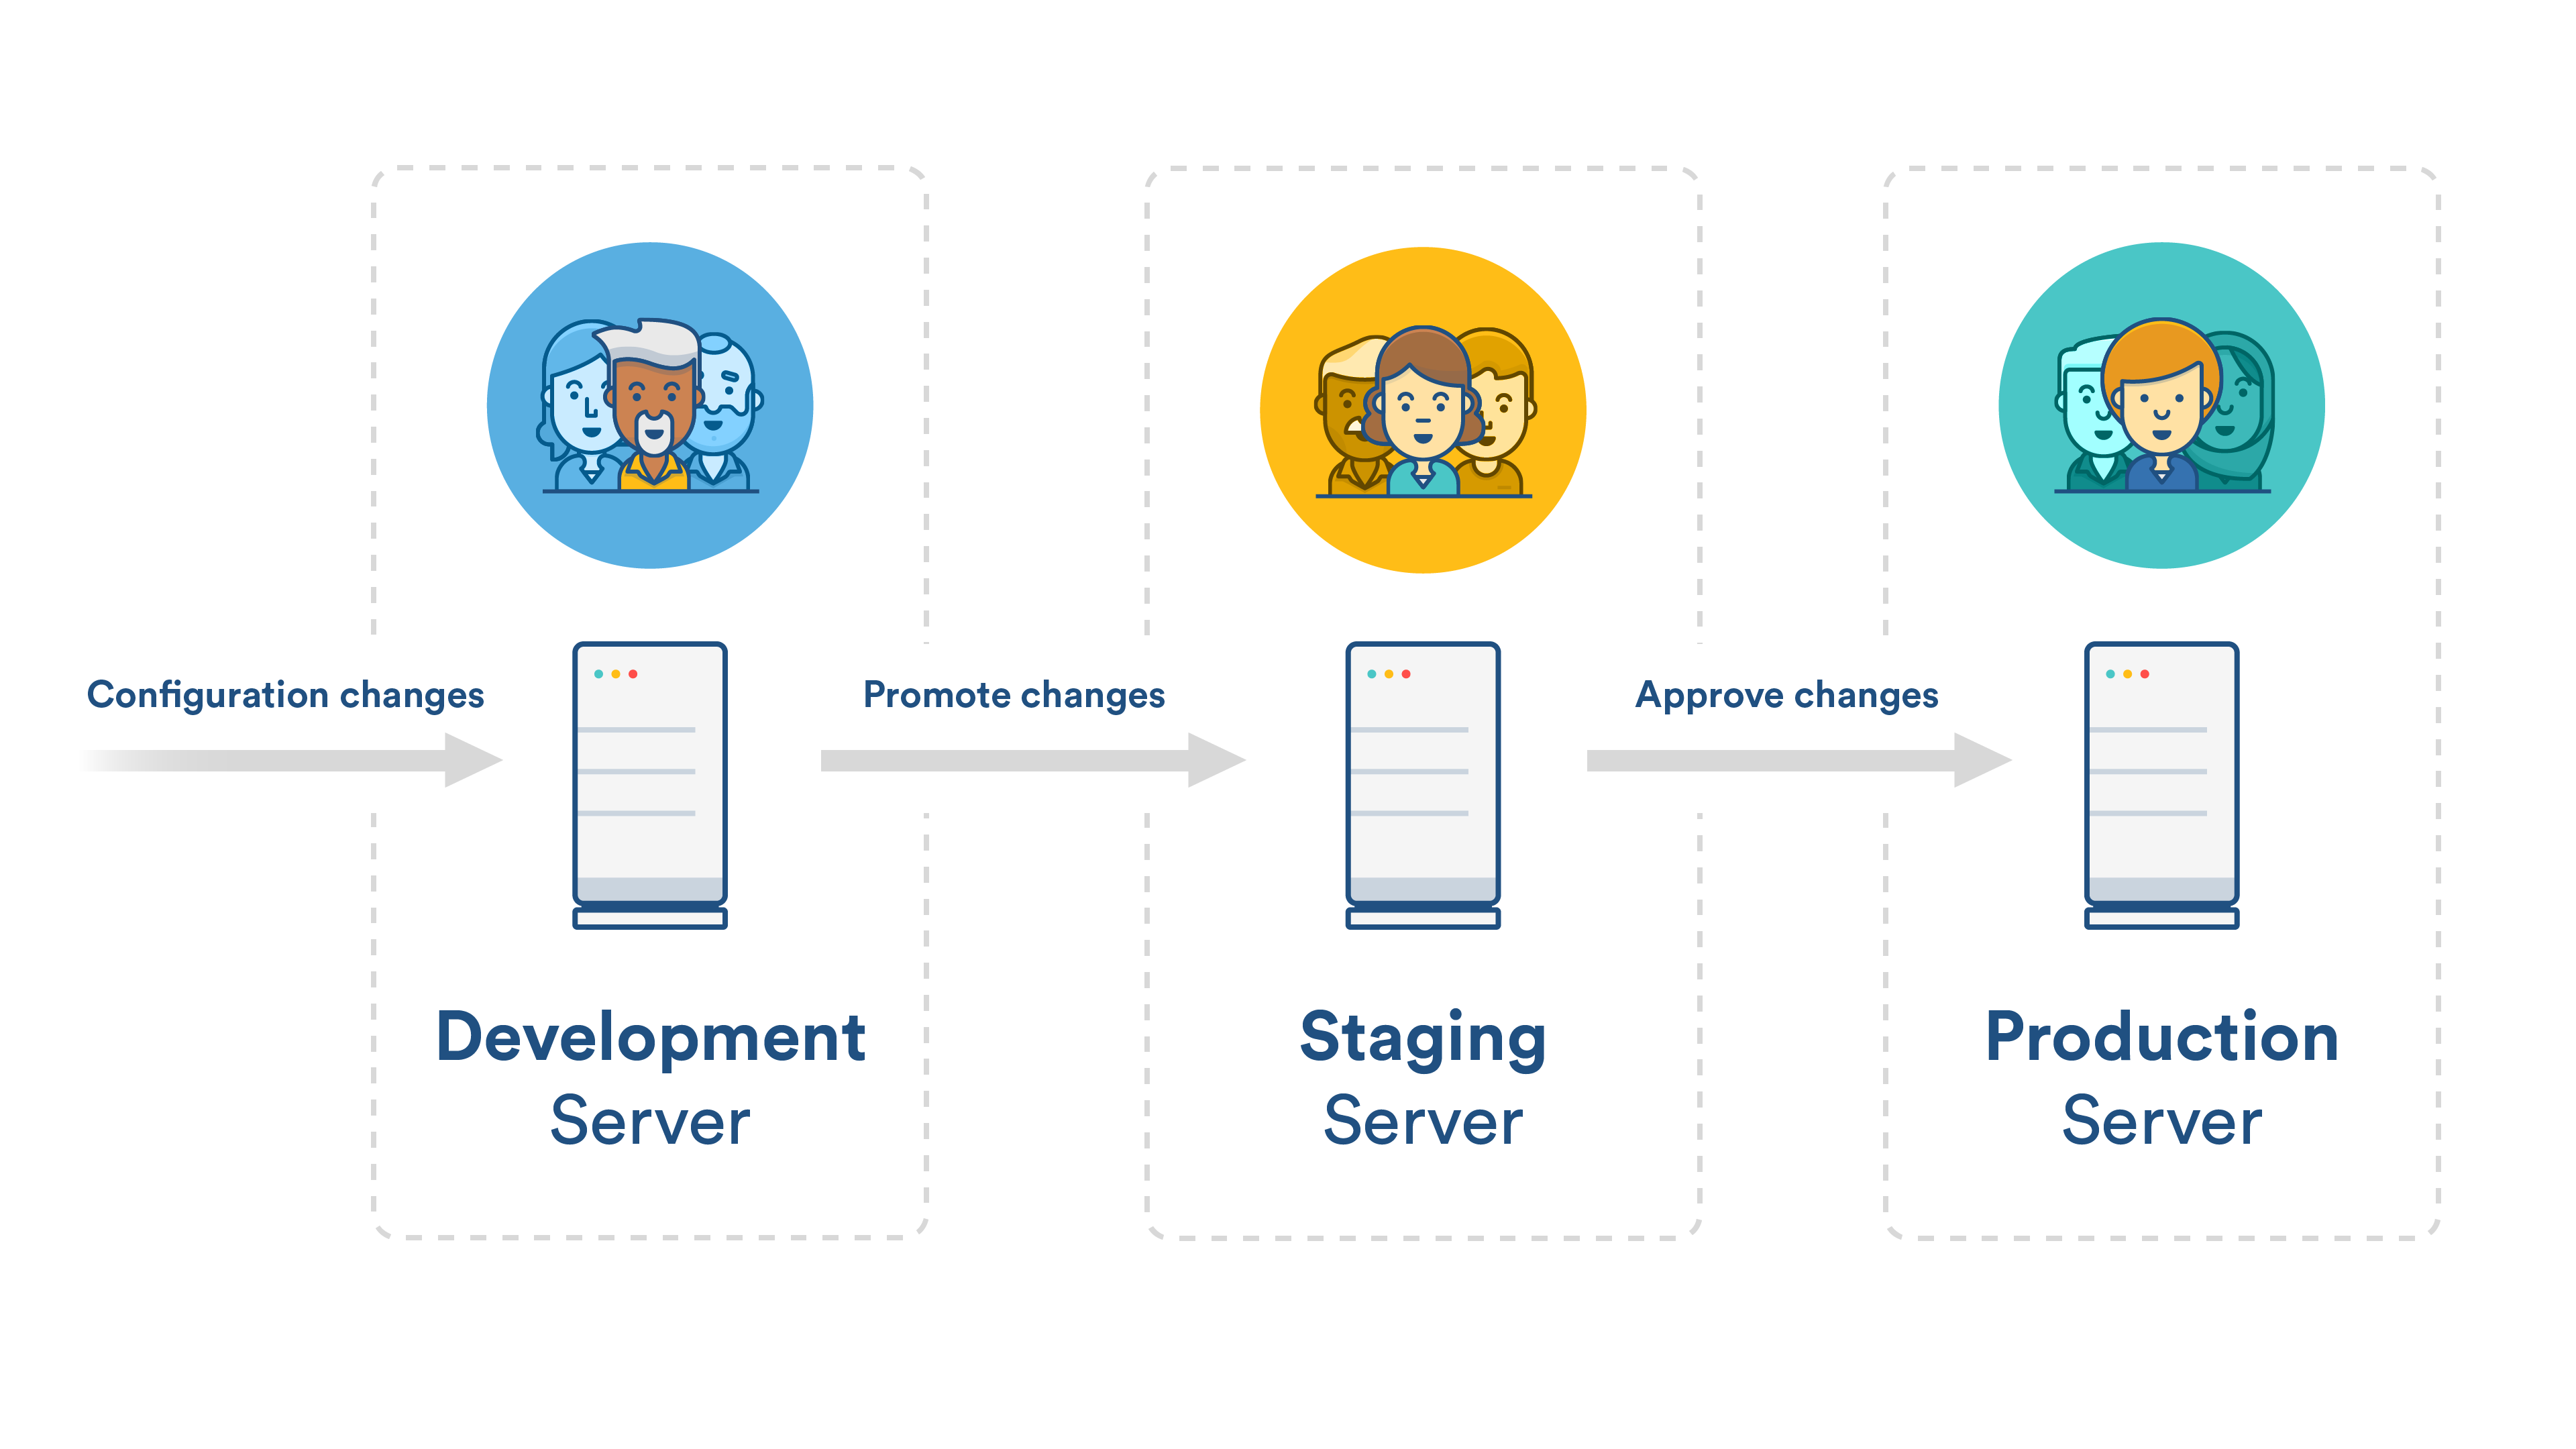
\includegraphics[scale=0.15]{software-flow.png}
    \caption{Fluxo do Sistema em Desenvolvimento\cite{atlassiansupport2018}}
    \label{fig:software-flow}
\end{figure}

\subsection{Estruturação no Projeto}
Para o projeto, foram construídos dois ambientes remotos, fora o ambiente final de produção que deve ficar na nuvem da USP. Os ambientes de desenvolvimento e homologação foram criados no Heroku, um serviço de plataforma (\textit{Platform as a Service} - \textbf{PaaS}), com os seguintes domínios:

\begin{itemize}
    \item Desenvolvimento: \href{https://tccapp-next-release.herokuapp.com}{https://tccapp-next-release.herokuapp.com}
    \item Homologação: \href{https://tccapp-staging.herokuapp.com}{https://tccapp-staging.herokuapp.com}
\end{itemize}

\section{Tecnologia Usada: Heroku\cite{lucasarthurfelgueiras2018}}

O Heroku é uma plataforma de computação em nuvem conhecida no mercado, com a possibilidade de subir aplicações nas linguagens Ruby, Node.js, Java, Python, Clojure, Scala, Go e PHP. O grande destaque do Heroku está na facilidade em subir uma aplicação com facilidade e de maneira gratuita, o que possibilita testar e validar ideias básicas antes de escalar de fato. A estrutura básica do Heroku funciona com o uso de \textit{dynos}, que servem tanto para hospedar sua aplicação principal quanto máquinas auxiliares para serviços externos e/ou paralelos.

\subsection{Funcionamento básico}

\begin{figure}[H]
  \centering
  \includegraphics[scale=0.20]{heroku-architecture.eps}
  \caption{Arquitetura Básica do Heroku\cite{safariheroku}}
  \label{fig:heroku-architecture}
\end{figure}

O funcionamento do Heroku consiste no uso de \textit{dynos} para hospedar as aplicações e nos \textit{routers} para tratar e encaminhas as requisições dos usuários. Além disso, o próprio Heroku disponibiliza extensões para gerenciar sua aplicação, como por exemplo o gerenciador de IP estático, ou o banco de dados necessário para a aplicação.

\subsection{Tarifação}

O Heroku possui um diferencial em relação à tarifação: possui um plano básico gratuito que possibilita testar aplicações de maneira fácil e sem dificuldades de expansão. Essencialmente, a cobrança do Heroku ocorre via uso de seus \textit{dynos}-hora. Além disso, há a cobrança pelas extensões usadas dentro da aplicação, onde, no geral, há um plano gratuito de testes ou até para projetos pequenos funcionarem com tranquilidade sem necessidades de escalabilidade.


\chapter{Metodologia de Trabalho}

\section{Processos de Levantamento de Requisitos}
\section{Divisão em Iterações}

\chapter{Especificação de Requisitos do Sistema}

\section{Pontos Levantados nas Reuniões}
\section{Requisitos Funcionais}
\section{Requisitos Não Funcionais}

\chapter{Projeto e Implementação}

\section{Elaboração e Estrutura do Sistema}
\section{Problemas Iniciais da Implementação}

\chapter{Teste e Validação}

\section{Validações}
\section{Testes Executados}
\section{Ambientes de Validação}

\chapter{Considerações Finais}
\section{Perspectivas}

\section{Resultados Alcançados}




% ========== Referências ==========
% --- IEEE ---
%	http://www.ctan.org/tex-archive/macros/latex/contrib/IEEEtran
%\bibliographystyle{IEEEbib}

% --- ABNT (requer ABNTeX 2) ---
%	http://www.ctan.org/tex-archive/macros/latex/contrib/abntex2
\bibliographystyle{abntex2-num}

\bibliography{refs}

% ========== Apêndices (opcional) ==========
\apendice
\chapter{Documento de Visão}

\section{Introdução}
\subsection{Finalidade e Visão Geral do Documento}

O documento tem como finalidade coletar informações e unificar os pontos de vista sobre o sistema de gerenciamento da disciplina de TCC, como as necessidades encontradas e as causas para tais necessidades.

\subsection{Referências}

O site do departamento, bem como o Tidia-AE serviram como referência auxiliar para entender melhor as soluções atuais.

\section{Posicionamento}
\subsection{Descrição do Problema}

\begin{table}[!htb]
    \centering
    \caption{Descrição básica do problema}
    \label{my-label}
    \resizebox{\textwidth}{!}{\begin{tabular}{|l|l|lll}
        \cline{1-2}
        O problema de         & alto tempo e esforço para gerenciar a disciplina de maneira manual    &  &  &  \\ \cline{1-2}
        afeta                 & orientadores, alunos e coordenadores da disciplina            &  &  &  \\ \cline{1-2}
        cujo impacto é        & demora e esforço para notas, dificuldade para integração entre envolvidos, problemas de demanda     &  &  &  \\ \cline{1-2}
        uma boa solução seria & automatizar o processo e integrar os orientadores no processo &  &  &  \\ \cline{1-2}
    \end{tabular}}
\end{table}

\subsection{Sentença de Posição do Produto}

\begin{table}[!htb]
    \centering
    \caption{Sentença básica de posição do produto}
    \label{my-label}
    \resizebox{\textwidth}{!}{\begin{tabular}{|l|l|lll}
        \cline{1-2}
        Para            & alunos, orientadores, coordenadores e técnicos                                                                  &  &  &  \\ \cline{1-2}
        Que             & cursam ou estão envolvidos diretamente                                                            &  &  &  \\ \cline{1-2}
        O sistema       & de gerenciamento dos TCC's                                                                                      &  &  &  \\ \cline{1-2}
        Que             & armazena os TCC's anteriores e gerencia o TCC atual, realizando avaliação e controlando entregas                                                             &  &  &  \\ \cline{1-2}
        Ao contrário do & processo semi-manual de gerenciamento da disciplina, do Tidia-AE e do Site institucional em Wordpress                                                             &  &  &  \\ \cline{1-2}
        O sistema       & permite um acompanhamento dos envolvidos, bem como serve de histórico para os trabalhos anteriores &  &  &  \\ \cline{1-2}
    \end{tabular}}
\end{table}


\section{Descrições dos Envolvidos e Usuários}
\subsection{Resumo dos envolvidos}

Há alguns usuários que não estão diretamente envolvidos com o sistema, mas podem ser beneficiados ou interferem no sistema a ser desenvolvido:

\begin{itemize}
    \item Infraestrutura: Irá aplicar restrições tecnológicas e de negócio dado o ambiente desenvolvido.
    \item Secretaria do Departamento: Nem todos os integrantes irão usar o sistema, mas serão beneficiados pela automação de alguns processos internos da disciplina, diminuindo a demanda recorrente sobre a equipe, vide o fato deles gerenciarem as entregas das avaliações durante o processo.
\end{itemize}

\subsection{Resumo dos usuários}

Há diversos usuários que serão diretamente beneficiados com o sistema. São eles:

\begin{itemize}
    \item Coordenador: Responsáveis por administrarem as disciplinas de TCC 1 e 2 para os cursos de Engenharia de Computação Semestrais e Quadrimestrais.
    \item Orientador: Responsável por construír com os alunos a monografia.
    \item Técnico de Operação: Responsável por administrar novas funcionalidades futuras do sistema.
    \item Técnico do Evento: Responsável por cuidar da parte de infraestrutura dos eventos a serem realizados.
    \item Alunos: Os cursantes das disciplinas de TCC 1 e 2.
    \item Avaliador Teórico: Avaliam os projetos realizados, durante a banca de defesa.
    \item Avaliador Prático: Avaliam os projetos realizados, durante a feira de projetos de formatura.
\end{itemize}

\subsection{Representantes dos usuários}

Foram escolhidos representantes dos perfis citados acima, de maneira a facilitar conversas durante a especificação do documento.

\begin{itemize}
    \item João Batista/Paulo Cugnasca: Coordenadores das duas disciplinas.
    \item Edson Gomi: Professor orientador
    \item Selma: Avaliadora Teórica
    \item Nilton: Técnico do Evento
    \item Michelet: Técnico de Operação
    \item Fábio Levy: Responsável pela infraestrutura de hospedagem.
    \item Bruno Albertini: Responsável pela infraestrutura de hospedagem.
    \item Ex-aluno: Processo do lado do aluno cursante da disciplina.
\end{itemize}

\subsection{Ambiente do usuário}

Para o processo em questão, podemos reforçar alguns pontos importantes:

\begin{itemize}
    \item São 2 professores coordenadores, 2 técnicos, cerca de 50 alunos por ano de TCC e cerca de 20 professores orientadores do departamento de PCS.
    \item O ciclo da disciplinas de TCC dura 1 ano, sendo metade do tempo de especificação e metade de implementação.
    \item Atualmente, há a plataforma Tidia-AE existente para administrar as disciplinas. Porém, ela serve apenas como repositório de arquivos, sem a participação direta dos orientadores e sem infraestrutura de automação e comunicação rápida entre os envolvidos.
    \item Além disso, há o site do departamento, onde ficam as monografias mais recentes, também como simples repositório de arquivos.
\end{itemize}

\subsection{Principais necessidades do usuário}

Diversas necessidades foram encontradas, sendo agrupadas, estudadas e propostas soluções para atendê-las. A lista das necessidades encontradas está a seguir:

\begin{table}[!htb]
  \centering
  \caption{Necessidades encontradas}
  \label{my-label}
  \resizebox{\textwidth}{!}{\begin{tabular}{|l|l|l|l|}
    \hline
    Necessidade                                                                         & Prior. & Sol.Atual         & Sol. Proposta                                                \\ \hline
    Orientador, coordenadores e alunos têm dificuldades em manter contato              & 1      & E-mail, reuniões  & Colocar os orientadores nas entregas                         \\ \hline
    Busca de monografias antigas é complexa.                                            & 2      & Site do PCS       & Criar repositório de monografias finalizadas                 \\ \hline
    O processo de gerenciar empresas participantes é extremamente manual.               & 7      & Conversas         & Integrar empresas às monografias a serem avaliadas           \\ \hline
    Avaliadores têm dificuldade em acessar monografias.                                 & 4      & E-mail            & Permitir monografia de fácil acesso no sistema               \\ \hline
    Avaliação dos projetos é de maneira manual.                                         & 5      & Papel             & Permitir avaliação pelo sistema, inclusive de maneira mobile \\ \hline
    Encontrar temas e alunos e propor temas é um processo manual.                       & 9      & E-mail, conversas & Permitir alunos e orientadores proporem temas no sistema     \\ \hline
    O gerenciamento de recursos pela parte do técnico é depende dos alunos solicitarem. & 8      & E-mail, pen drive & Automatizar as demandas para os técnicos providenciarem      \\ \hline
    O processo de montagem da banca de TCC é manual.                                    & 6      & E-mail, conversas & Permitir montagem de bancas pelo sistema                     \\ \hline
    Fechar as notas finais é um processo exaustivo e com curto prazo.                   & 3      & Papel             & Automatizar o cálculo das notas finais                       \\ \hline
  \end{tabular}}
\end{table}

\subsection{Alternativas e concorrência}
\begin{itemize}
    \item Tidia-AE: Entregas pontuais, com acesso apenas aos integrantes do grupo e aos coordenadores da disciplina. Os orientadores ficam de fora das entregas principais, cabendo aos alunos realizarem essa comunicação de maneira extra-oficial.
    \item Moodle: Plataforma aberta conhecida no mercado para gerenciamento de disciplinas em geral. Serve para construir grupos e até incluir orientadores, porém não é uma alternativa simples e não possui funcionalidades de busca avançada.
    \item Site PCS (Wordpress): Apenas resultado final, de maneira pública, sem integração dos envolvidos no projeto.
\end{itemize}

\section{Visão Geral do Produto}
\subsection{Perspectiva do Produto}
O produto tem como missão automatizar o processo já existente para a disciplina, pois muitas funcionalidades propostas são realizadas de maneira manual ou simplificada, o que demanda muito tempo e esforço dos coordenadores e orientadores, tornando o processo frágil. Além disso, depende da iniciativa de todos os envolvidos, pois todo o processo de comunicação orientador-aluno é feito de maneira isolada do processo coordenador-aluno e coordenador-orientador.

\subsection{Suposições e Dependências}
A principal dependência encontrada é que o serviço deve ser hospedado na infraestrutura interna da Universidade de São Paulo, o que afetará a maneira como o produto será desenvolvido.
  
\section{Recursos do Produto}
O produto a ser desenvolvido deve atender as necessidades descritas anteriormente, ou seja, possíveis conteúdos interessantes são:

\begin{itemize}
    \item Facilitar comunicação orientador/coordenadores, permitindo que eles vejam todas as entregas dos alunos e validem, quando necessário.
    \item Buscar, de maneira pública, as monografias antigas, usando filtros e busca textual.
    \item Incluir avaliadores da feira no sistema para acompanhar monografias correntes.
    \item Permitir avaliação tanto da banca como da feira (com as empresas), permitindo acesso prévio ao conteúdo e facilitando a avaliação (de preferência na plataforma mobile).
    \item Permitir que orientadores, alunos e empresas proponham temas e consigam combinar grupos para realizar as propostas.
    \item Permitir aos técnicos gerenciarem recursos necessários para as apresentações (imprimir apresentações sem necessidade do aluno entregar arquivos via pen drive, por exemplo)
    \item Permitir a montagem de bancas de TCC, convidando os envolvidos e facilitando o acesso ao resultado final do aluno.
\end{itemize}
  
\section{Outros requisitos do produto}
Como principais requisitos não-funcionais importantes, vale ressaltar:

\begin{itemize}
    \item Confiabilidade: O sistema deve permanecer funcional durante as avaliações finais do curso, pois são cruciais para o bom andamento da matéria.
    \item Segurança: Os acessos às monografias em andamento devem ser apenas aos envolvidos diretos do trabalho. Além disso, as empresas só podem acessar o resultado final não revisado, para fins de avaliação.
    \item Usabilidade: O sistema deve ser bem intuitivo e de aprendizagem fácil, pelo tempo curto dos envolvidos na feira e pela mobilidade envolvida (avaliações pelo celular, por exemplo).
\end{itemize}

\chapter{Diagramas BPMN}

\section{Introdução}

Os diagramas de Modelo e Notação de Processos de Negócio (Business Process Model and Notation - BPMN) servem para modelar um processo de negócio de maneira a unificar a visão sobre aquele processo e encontrar possíveis otimizações para o mesmo processo.

Para o trabalho em questão, foram usados os diagramas para levantar o processo antes do sistema e após o sistema, assim evidenciamos a presença dele e em que ele ajuda no processo da disciplina.

Para este projeto, foi usada a ferramenta Draw.io\cite{drawio}, para elaborar os diagramas BPMN dos processos citados. Apesar de não ser uma ferramenta específica para esse tipo de diagrama, é uma ferramenta de diagramação simples e que possui bibliotecas de diversos tipos de diagramas, inclusive os de BPMN.

\section{Processo antes do Sistema}

Os diagramas BPMN foram gerados com base nas entrevistas realizadas durante o processo de levantamento de requisitos. Os resultados estão a seguir:

\clearpage
\subsection{TCC 1}

\begin{figure}[H]
    \centering
    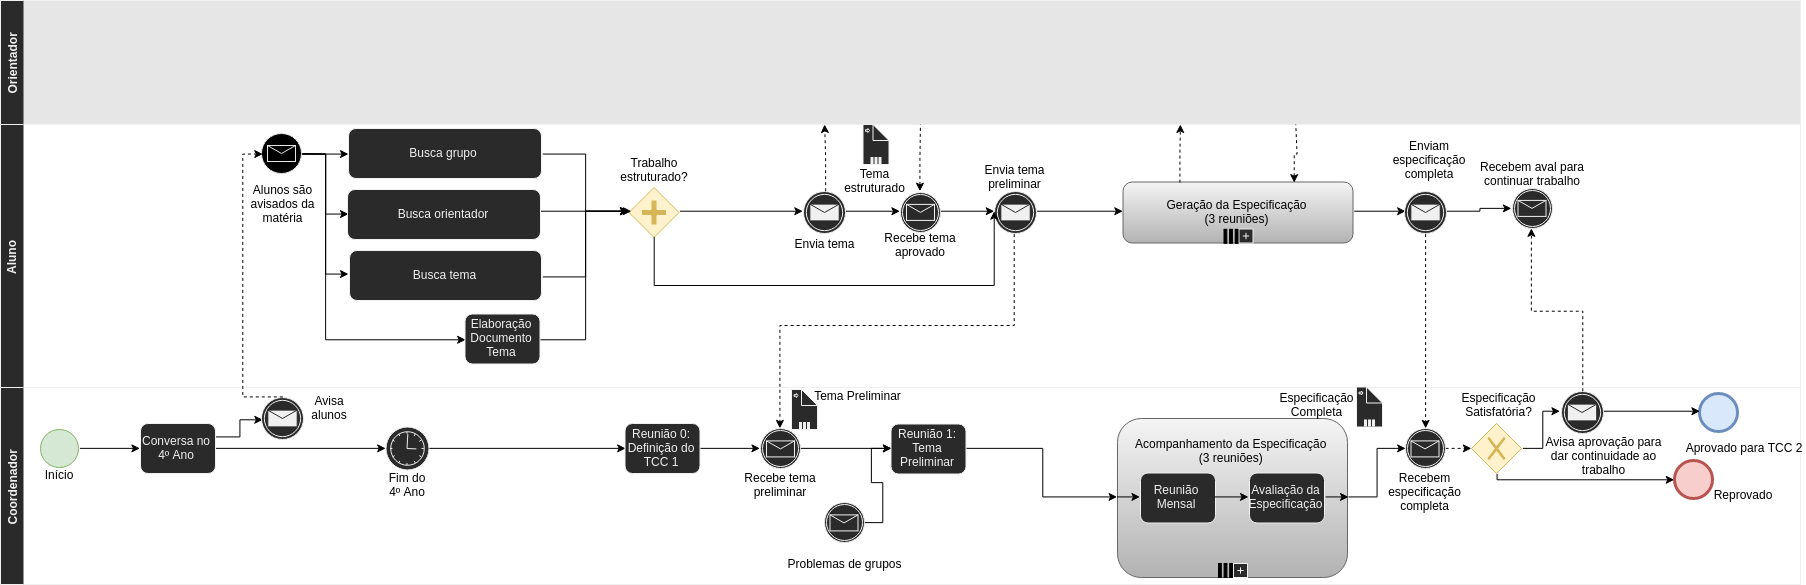
\includegraphics[angle=90, origin=c, scale=0.35]{bpmn-tcc1.png}
    \caption{Diagrama BPMN para a disciplina de TCC 1}
    \label{fig:bpmn-tcc1}
\end{figure}

\subsection{TCC 2}

\begin{figure}[H]
    \centering
    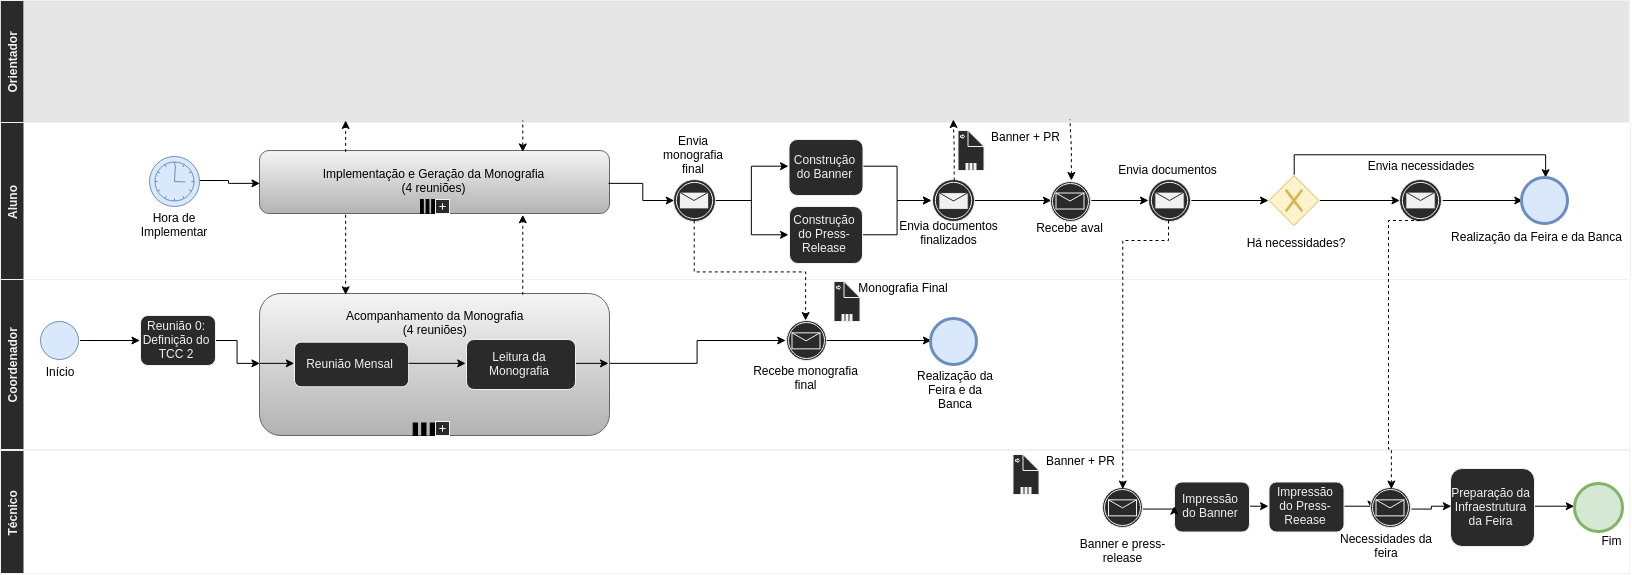
\includegraphics[angle=90, origin=c, scale=0.35]{bpmn-tcc2.png}
    \caption{Diagrama BPMN para a disciplina de TCC 2, antes dos eventos finais}
    \label{fig:bpmn-tcc2}
\end{figure}

\subsection{Banca e Feira}

\begin{figure}[H]
    \centering
    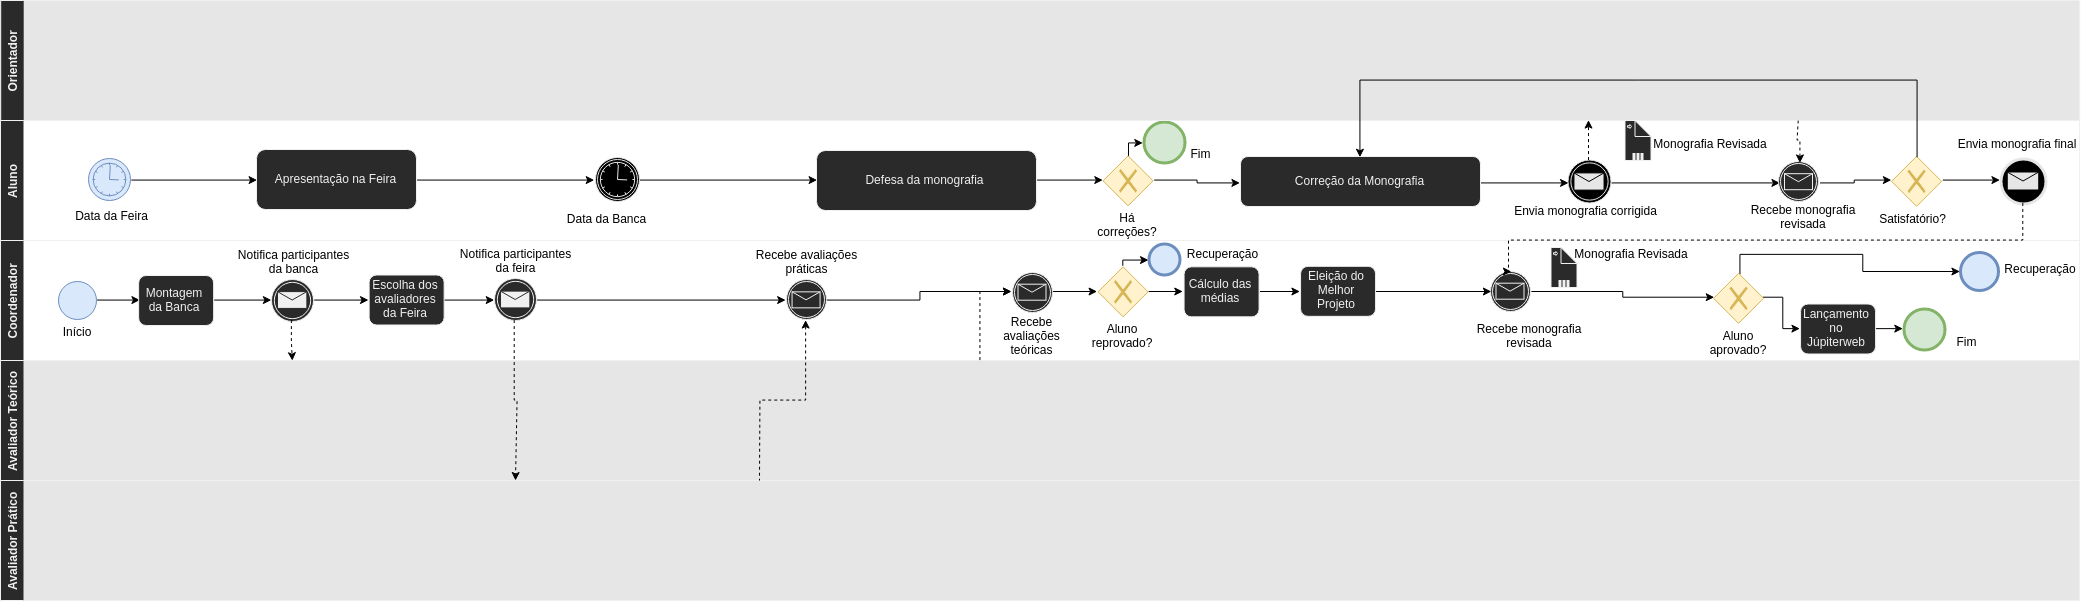
\includegraphics[angle=90, origin=c, scale=0.3]{bpmn-banca-feira.png}
    \caption{Diagrama BPMN para os eventos de banca e feira}
    \label{fig:bpmn-banca-feira}
\end{figure}

\subsection{Recuperação}

\begin{figure}[H]
    \centering
    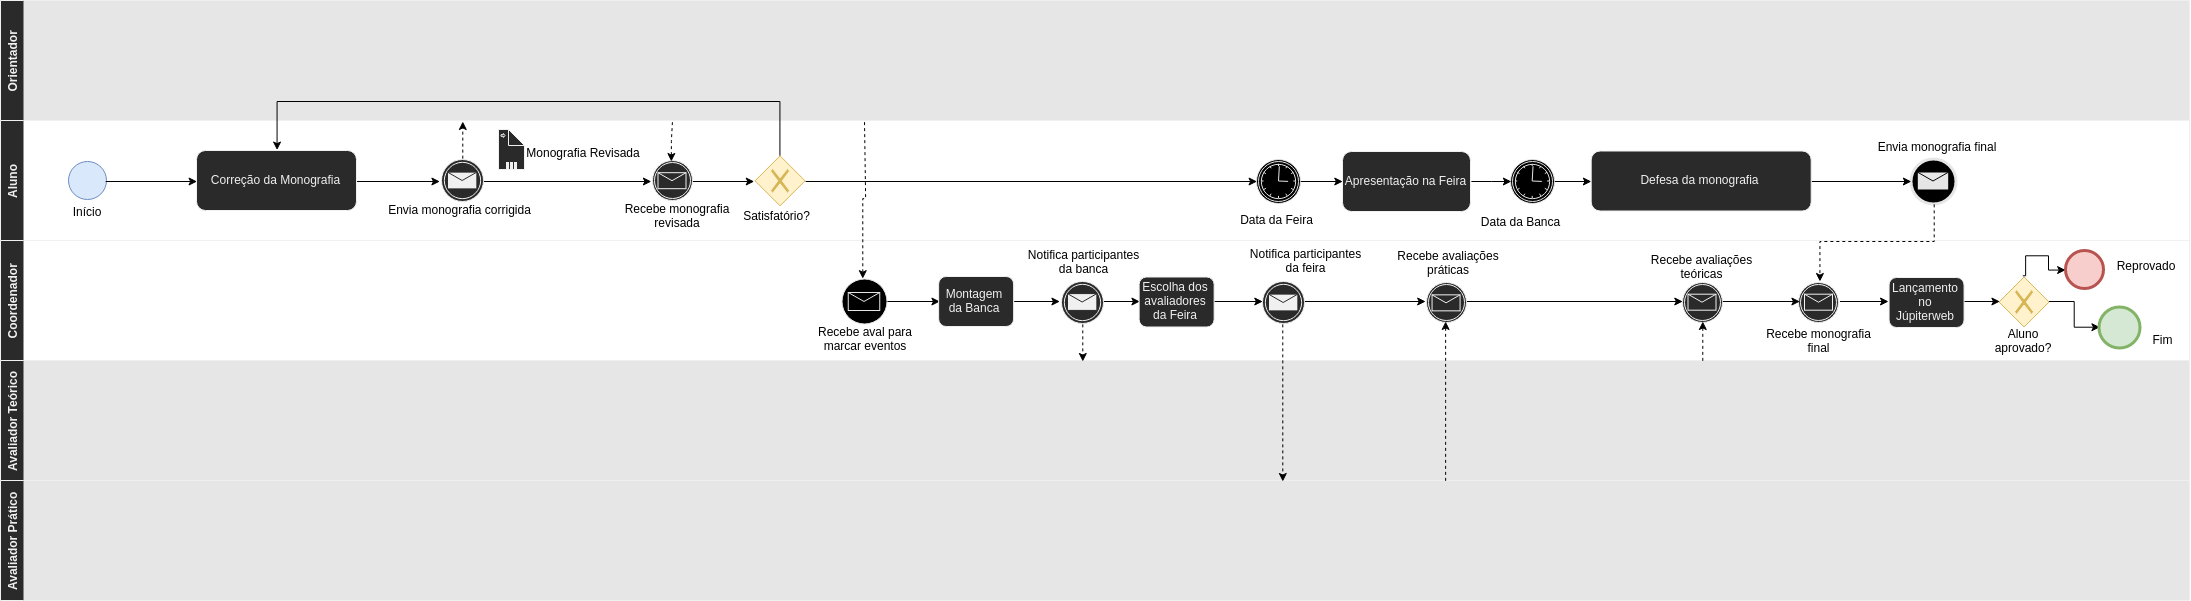
\includegraphics[angle=90, origin=c, scale=0.3]{bpmn-rec.png}
    \caption{Diagrama BPMN para a recuperação da disciplina de TCC 2}
    \label{fig:bpmn-rec}
\end{figure}

\section{Processo com o Sistema}

Já esses diagramas BPMN foram gerados com base no documento de visão, elaborado após o processo de levantamento de requisitos. Os resultados estão a seguir:

TO-DO


\chapter{Casos de Uso}\label{chap:use-case-appendix}

\section{Introdução}

Neste apêndice consta os casos de uso escritos para o sistema em questão, usando o padrão explicado no capítulo de casos de uso\cite{funpar2001}.

\subsection{Cadastrar disciplinas}


\begin{enumerate}
    \item Breve Descrição


Coordenadores cadastram a disciplina, os alunos participantes e as atividades.


    \item Fluxo de Eventos

\begin{enumerate}
    \item Fluxo Básico

\begin{itemize}
    \item Coordenador insere disciplina, com os seguintes dados:

\begin{itemize}
    \item Modalidade (Sem/Quad)

    \item Data de início e data de término


\end{itemize}
    \item Coordenador importa planilha com alunos participantes, com os seguintes dados dos alunos

\begin{itemize}
    \item Nome

    \item E-mail

    \item Nº USP


\end{itemize}
    \item Coordenador insere uma nova atividade da disciplina, com os seguintes dados

\begin{itemize}
    \item Nome

    \item Data de entrega e arquivos relacionados

    \item Peso da atividade


\end{itemize}
    \item Sistema salva alunos novos, dispara e-mail ao aluno com seu acesso (login e senha) e vincula os existentes à disciplina e salva a disciplina
\end{itemize}

    \item Fluxos Alternativos

\begin{enumerate}
    \item Data de início é posterior a de término

\begin{enumerate}
    \item Sistema exibe novamente tela de cadastro da disciplina, alertando sobre erro


\end{enumerate}
    \item E-mail é inválido

\begin{enumerate}
    \item Sistema exibe novamente tela de cadastro da disciplina, alertando sobre erro


\end{enumerate}
    \item E-mail retornou

\begin{enumerate}
    \item Sistema envia e-mail ao coordenador com o aluno problemático




\end{enumerate}
\end{enumerate}
\end{enumerate}
    \item Requisitos Especiais


Não há


    \item Pré-condição


Coordenador deve estar logado


    \item Pós-condição

    Não há
\end{enumerate}

\subsection{Editar disciplinas}


\begin{enumerate}
    \item Breve Descrição


Coordenadores editam disciplinas, cadastrando atividades, editando alunos etc.


    \item Fluxo de Eventos

\begin{enumerate}
    \item Fluxo Básico

\begin{itemize}
    \item Coordenador edita início e término da disciplina, alunos participantes, com novos alunos ou removendo os já participantes

    \item Coordenador insere uma nova atividade da disciplina, com os seguintes dados

\begin{itemize}
    \item Nome

    \item Data de entrega

    \item Arquivos relacionados

    \item Peso da atividade


\end{itemize}
    \item Sistema salva novas atividades e as mudanças da disciplina
\end{itemize}

    \item Fluxos Alternativos



\end{enumerate}
    \item Requisitos Especiais


Não há


    \item Pré-condição


Coordenador deve estar logado


    \item Pós-condição

    Não há
\end{enumerate}

\subsection{Cadastrar professores}


\begin{enumerate}
    \item Breve Descrição


Coordenadores cadastram professores do departamento que podem orientar/co-orientar.


    \item Fluxo de Eventos

\begin{enumerate}
    \item Fluxo Básico

\begin{itemize}
    \item Coordenador insere os dados do professor

\begin{itemize}
    \item Nome 

    \item Número USP

    \item E-mail


\end{itemize}
    \item Sistema salva o professor, disparando e-mail para o professor cadastrado
\end{itemize}


    \item Fluxos Alternativos



\end{enumerate}
    \item Requisitos Especiais


Não há


    \item Pré-condição


Coordenador deve estar logado


    \item Pós-condição

    Não há
\end{enumerate}




















\subsection{Cadastrar grupos de trabalhos}


\begin{enumerate}
    \item Breve Descrição


Coordenadores cadastram os grupos com os temas e os orientadores, com a confirmação da participação do orientador no grupo.


    \item Fluxo de Eventos

\begin{enumerate}
    \item Fluxo Básico

\begin{itemize}
    \item Coordenador insere os dados do grupo

\begin{itemize}
    \item Título

    \item Alunos

    \item Orientador

    \item Co-orientador


\end{itemize}
    \item Sistema salva grupo e envia e-mail para o orientador, co-orientador e alunos

    \item Orientador valida participação no grupo

    \item Co-orientador valida participação no grupo
\end{itemize}


    \item Fluxos Alternativos

\begin{enumerate}
    \item Grupo não tem orientador

\begin{enumerate}
    \item Sistema cadastra grupo, enviando e-mail para os alunos com o aviso de urgência na escolha do orientador


\end{enumerate}
    \item Grupo não tem aluno

\begin{enumerate}
    \item Sistema retorna para a tela de cadastro de grupo, avisando sobre o erro de ausência de alunos
\end{enumerate}
\end{enumerate}


    \item Requisitos Especiais


Não há


    \item Pré-condição


Coordenador deve estar logado, alunos, orientadores e co-orientadores cadastrados


    \item Pós-condição

    Grupo confirmado
\end{enumerate}
\end{enumerate}

\subsection{Login}


\begin{enumerate}
    \item Breve Descrição


Alunos, Orientadores, Co-orientadores e Coordenadores acessam sistema de maneira tradicional ou via Senha Única USP (para pertencentes à USP).


    \item Fluxo de Eventos

\begin{enumerate}
    \item Fluxo Básico

\begin{itemize}
    \item Sistema mostra campos de login e senha

    \item Usuário insere seu e-mail e sua senha

    \item Sistema valida e-mail e senha

    \item Usuário acessa sistema
\end{itemize}


    \item Fluxos Alternativos

\begin{enumerate}
    \item Usuário erra credenciais

\begin{enumerate}
    \item Sistema retorna para tela de acesso ao sistema, exibindo mensagem de erro

    \item Retorna normalmente à situação de mostrar campos de login e senha


\end{enumerate}
    \item Usuário realiza login pela Senha Única da USP

\begin{enumerate}
    \item Usuário seleciona $``$Acessar pela Senha Única USP$"$ 

    \item Usuário é redirecionado para os sistemas USP

    \item Retorna para a situação de acesso ao sistema
\end{enumerate}
\end{enumerate}


    \item Requisitos Especiais


Integração via Shibboleth com os Sistemas USP


    \item Pré-condição


Não há


    \item Pós-condição

    Usuário dentro do sistema
\end{enumerate}
\end{enumerate}


\subsection{Entregar atividade}


\begin{enumerate}
    \item Breve Descrição


Alunos submetem no Google Drive arquivos da atividade para a leitura do orientador, co-orientador e coordenadores. Orientador e co-orientador revisam e dão seu aval de aprovação com a documentação.


    \item Fluxo de Eventos

\begin{enumerate}
    \item Fluxo Básico

\begin{itemize}
    \item Aluno submete arquivos nos respectivos espaços de atividades, que são carregados no Google Drive e deixa comentários adicionais sobre a entrega

    \item Sistema salva a entrega com o status da entrega da atividade para $``$Não avaliada$"$ 

    \item Sistema envia e-mail para Orientador e Co-orientador avisando de submissão

    \item Orientador baixa documentos submetidos

    \item Orientador avalia a entrega, faz comentários aos alunos e comentários exclusivos à coordenação com notas

    \item Sistema salva entrega e dispara e-mail com o resultado da avaliação para os alunos
\end{itemize}


    \item Fluxos Alternativos

\begin{enumerate}
    \item Data de submissão expirou (1)

\begin{enumerate}
    \item Aluno não consegue interagir com atividade, encerrando fluxo


\end{enumerate}
    \item Co-orientador realiza fluxo de revisão, antes do Orientador (4)

\begin{enumerate}
    \item Passos 5 - 7 ocorrem normalmente, trocando Orientador por Co-orientador


\end{enumerate}
    \item Co-orientador realiza fluxo de revisão, após Orientador (8)

\begin{enumerate}
    \item Sistema exibe detalhes da entrega, porém não permite edições do lado do Co-orientador, encerrando fluxo


\end{enumerate}
    \item Aluno submete nova entrega da atividade após ter feito uma submissão (1)

\begin{enumerate}
    \item Aluno vê status da avaliação

    \item Aluno realiza nova entrega da atividade, repetindo o caso de uso


\end{enumerate}
    \item Aluno submete entrega da atividade quando alguém do grupo já submeteu (1)

\begin{enumerate}
    \item Sistema exibe detalhes da entrega já realizada

    \item Aluno pode realizar nova entrega da atividade, passando por cima da entrega anterior e repetindo o caso de uso
\end{enumerate}
\end{enumerate}

    \item Requisitos Especiais


Não há


    \item Pré-condição


Atores devem estar autenticados e atividade deve estar cadastrada no sistema


    \item Pós-condição
    
    Não há
\end{enumerate}
\end{enumerate}


\subsection{Construir bancas práticas}


\begin{enumerate}
    \item Breve Descrição


Coordenadores selecionam os participantes da banca prática, já cadastrados no sistema, e os notifica com comentários sobre o evento.


    \item Fluxo de Eventos

\begin{enumerate}
    \item Fluxo Básico

\begin{itemize}
    \item Coordenador informa o dia da feira, a disciplina correspondente e as salas disponíveis para o evento, além de determinar o peso da avaliação da banca

    \item Sistema salva evento

    \item Coordenador seleciona evento recém criado.

    \item Sistema lista grupos do evento.

    \item Coordenador seleciona o grupo que deseja atribuir a sala e os convidados.

    \item Coordenador seleciona os convidados que avaliarão o grupo

    \item Sistema salva banca e envia e-mail para os convidados externos, avisando-os sobre sua participação

    \item Convidado acessa sistema e confirma participação na banca
\end{itemize}

    \item Fluxos Alternativos

Não há

\end{enumerate}
    \item Requisitos Especiais


Não há


    \item Pré-condição


Atores devem estar autenticados e grupo de trabalho deve estar cadastrado no sistema


    \item Pós-condição

    Não há
\end{enumerate}












\subsection{Construir bancas teóricas}


\begin{enumerate}
    \item Breve Descrição


Coordenadores escolhem participantes da banca teórica do grupo, selecionam o presidente da banca, realizam o agendamento do horário, validando inconsistências (participante já possui horário ocupado) e notificam os participantes por e-mail.


    \item Fluxo de Eventos

\begin{enumerate}
    \item Fluxo Básico

\begin{itemize}
    \item Coordenador informa o dia da banca, a disciplina correspondente e as salas disponíveis para o evento

    \item Sistema salva evento

    \item Coordenador seleciona evento recém criado.

    \item Sistema lista grupos do evento.

    \item Coordenador seleciona o grupo que deseja atribuir a sala e os convidados.

    \item Coordenador seleciona os avaliadores da banca e o horário da avaliação. O orientador é um dos pré-selecionados por padrão
\end{itemize}

    \item Fluxos Alternativos

\begin{enumerate}
    \item Convidado externo já possui banca nesse dia e horário

\begin{enumerate}
    \item Sistema barra criação de banca, alertando sobre qual convidado já possui agenda ocupada


\end{enumerate}
    \item Sala está ocupada no horário selecionado

\begin{enumerate}
    \item Sistema barra criação de banca, alertando sobre qual sala já possui agenda ocupada
\end{enumerate}
\end{enumerate}

 \item Requisitos Especiais


Não há


    \item Pré-condição


Atores devem estar autenticados e grupo de trabalho deve estar cadastrado no sistema


    \item Pós-condição

    Não há
\end{enumerate}
\end{enumerate}


\subsection{Listar entregas}


\begin{enumerate}
    \item Breve Descrição


Técnicos recebem os arquivos de impressão, com normalização do título, separados por grupo.


    \item Fluxo de Eventos

\begin{enumerate}
    \item Fluxo Básico

\begin{itemize}
    \item Coordenador lista todas as entregas finais de impressão (\textit{banner} e \textit{press-release})

    \item Sistema salva as listas de arquivos finais, com o nome normalizado e envia por e-mail para o técnico responsável
\end{itemize}

    \item Fluxos Alternativos

\begin{enumerate}
    \item Grupo de trabalho está com arquivo faltante

\begin{enumerate}
    \item Sistema envia e-mail para o grupo com entrega faltante, avisando para regularizar a situação com urgência.
\end{enumerate}
\end{enumerate}

    \item Requisitos Especiais


Não há


    \item Pré-condição


Atores devem estar autenticados e grupo de trabalho deve estar cadastrado no sistema


    \item Pós-condição

    Não há
\end{enumerate}
\end{enumerate}

\subsection{Listar necessidades adicionais}


\begin{enumerate}
    \item Breve Descrição


Técnicos recebem necessidades adicionais revisadas pelos orientadores, separadas por grupo.


    \item Fluxo de Eventos

\begin{enumerate}
    \item Fluxo Básico

\begin{itemize}
    \item Coordenador lista todos os comentários das entregas finais

    \item Sistema salva a lista de comentários e a envia por e-mail para o técnico responsável
\end{itemize}

    \item Fluxos Alternativos



\end{enumerate}
    \item Requisitos Especiais


Não há


    \item Pré-condição


Atores devem estar autenticados e grupo de trabalho deve estar cadastrado no sistema


    \item Pós-condição

    Não há
\end{enumerate}






















\subsection{Avaliar projetos práticos}


\begin{enumerate}
    \item Breve Descrição


Participantes da banca prática avaliam os projetos que estão envolvidos, limitando avaliações até o final do dia.


    \item Fluxo de Eventos

\begin{enumerate}
    \item Fluxo Básico

\begin{itemize}
    \item Convidado externo acessa espaço da banca, com detalhes do grupo e as entregas finais

    \item Convidado preenche os comentários e as notas de acordo com cada critério estabelecido para avaliação de bancas práticas

    \item Convidado salva avaliação
\end{itemize}

    \item Fluxos Alternativos

\begin{enumerate}
    \item Convidado tenta submeter avaliação em dia diferente ao da banca prática

\begin{enumerate}
    \item Avaliação é barrada, avisando o convidado de que a avaliação só pode ser feita exclusivamente no dia



\end{enumerate}
\end{enumerate}
\end{enumerate}
    \item Requisitos Especiais


Não há


    \item Pré-condição


Atores devem estar autenticados e grupo de trabalho deve estar cadastrado no sistema


    \item Pós-condição

    Não há
\end{enumerate}
















\subsection{Avaliar monografias teóricas}


\begin{enumerate}
    \item Breve Descrição


Participantes da banca teórica avaliam as monografias que estão envolvidas, gerando comentários e definindo o status do trabalho (aprovado, aprovado com correções, recuperação e reprovado), limitando avaliações até o final do dia.


    \item Fluxo de Eventos

\begin{enumerate}
    \item Fluxo Básico

\begin{itemize}
    \item Participante da banca acessa espaço da banca, com detalhes do grupo e as entregas parciais e finais.

    \item Participante preenche os comentários e as notas de acordo com cada critério estabelecido para avaliação de bancas teóricas

    \item Participante salva avaliação, com seu parecer para aprovação da monografia

    \item Presidente da banca vê avaliações dos outros envolvidos e determina o parecer final para a banca, com comentários para o grupo
\end{itemize}

    \item Fluxos Alternativos

Não há



\end{enumerate}
    \item Requisitos Especiais


Não há


    \item Pré-condição


Atores devem estar autenticados e grupo de trabalho deve estar cadastrado no sistema


    \item Pós-condição

    Não há
\end{enumerate}


\subsection{Calcular nota final dos projetos}


\begin{enumerate}
    \item Breve Descrição


Coordenadores determinam a fórmula para calcular as notas finais, com base nas entregas parciais durante as duas disciplinas e o sistema calcula as notas finais de todos os grupos participantes.


    \item Fluxo de Eventos

\begin{enumerate}
    \item Fluxo Básico

\begin{itemize}
    \item Coordenador escolhe as duas disciplinas (TCC1 e TCC2), a banca teórica e a feira prática que deseja obter as entregas

    \item Sistema salva fórmula de avaliação

    \item Sistema lista todos os grupos, com as notas calculadas e os estados de avaliação de cada grupo
\end{itemize}

    \item Fluxos Alternativos

\begin{enumerate}
    \item Coordenador não preenche algum dos campos necessários

\begin{enumerate}
    \item Sistema barra criação de fórmula de avaliação, avisando os campos faltantes


\end{enumerate}
    \item Grupo tem alguma avaliação faltante

\begin{enumerate}
    \item Sistema exibe grupo, mas com campo de Não Avaliado


\end{enumerate}
    \item Grupo vai para recuperação na avaliação da banca teórica

\begin{enumerate}
    \item A nota calculada é a nota da banca teórica, passando todas as outras avaliações realizadas ao longo das disciplinas


\end{enumerate}
    \item Grupo é reprovado na avaliação da banca teórica

\begin{enumerate}
    \item A nota calculada é a nota da banca teórica, passando todas as outras avaliações realizadas ao longo das disciplinas

Não há



\end{enumerate}
\end{enumerate}
\end{enumerate}
    \item Requisitos Especiais


Não há


    \item Pré-condição


Atores devem estar autenticados e grupo de trabalho deve estar cadastrado no sistema


    \item Pós-condição

    Não há
\end{enumerate}


% ========== Anexos (opcional) ==========
\anexo

\end{document}
